\documentclass[tikz,border=10pt]{standalone}
\usepackage{tikz}
\usepackage{amsmath,amssymb}
\usetikzlibrary{automata,backgrounds,shapes,arrows,positioning,calc,fit}

% Custom commands
\newcommand{\push}[1][]{\mathsf{push}_{#1}}
\newcommand{\pop}[1][]{\mathsf{pop}_{#1}}

\begin{document}
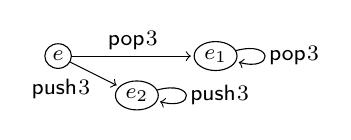
\begin{tikzpicture}[state/.style={draw,ellipse}, shorten >=1pt, node distance=2cm, on grid, auto,every node/.style={font=\footnotesize},inner sep=.05cm]
  % States for the \push{3}^*;\pop{3}^*
  \node[state] (q1) at (1,0) {$e$};
  \node[state] (q2) [right=of q1] {$e_1$};
  \node[state] (q3) at (2,-0.5){$e_2$};

  % Arrows for the \push{3}^*;\pop{3}^*
  \path[->]
    (q1) edge node {$\pop{3}$} (q2)
    (q1) edge node [swap] {$\push{3}$} (q3)
    (q2) edge[loop  right] node {$\pop{3}$} ()
    (q3) edge[loop  right] node {$\push{3}$} ();
\end{tikzpicture}
\end{document}